\documentclass[../../thesis.tex]{subfiles}

\begin{document}
\begin{figure}[htb]
    \centering
    \subfloat[]{
    \tikzsetnextfilename{cp_cond_evap}
        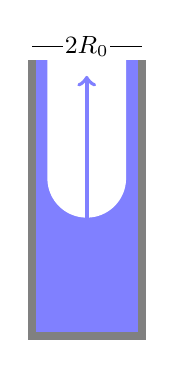
\begin{tikzpicture}[every node/.style = {font = \small},
                        pore/.style = {line width = 0.1cm, color = gray},
                        film/.style = {line width = 0.1cm, color = blue!50},
                        thick_film/.style = {line width = 0.3cm, color = blue!50},
                        graph_label/.style={color = gray, line width = 0.05cm},
                        pore_collapse/.style = {color = blue!50, line width = 0.07cm, ->},
                        MyArrow/.style={single arrow, draw, minimum width=8mm, minimum height=3mm,
                        inner sep=0mm, single arrow head extend=1mm},
                        fontscale/.style = {font=\relsize{#1}},
                        arrowstyle/.style = {scale=2},
                        MyArrow/.style={single arrow, draw, minimum width=8mm, minimum height=5mm, inner sep=0mm, single arrow head extend=1mm},
                        directed/.style={postaction={decorate,decoration={markings, mark=at position .65 with {\arrow[arrowstyle]{stealth}}}}}]
            \pgfdeclarelayer{bg}    % declare background layer
            \pgfdeclarelayer{bbg}    % declare backbackground layer
            \pgfsetlayers{bbg,bg,main}  % set the order of the layers (main is the standard layer)
            \begin{scope}
            \draw (0.4,3.67) -- (0,3.67);
            \draw (1,3.67) -- (1.4,3.67);
            \node at (0.7,3.67) {$2R_0$};
                \draw[pore] (0,3.5) -- (0,0) -- (0 + 1.4,0) -- (0 + 1.4,3.5);
                \begin{pgfonlayer}{bg}
                    \fill[blue!50] (0.01,0) -- (0.01,3.5)  -- (1.39,3.5) -- (1.39,0) -- cycle ;
                    \fill[white] (1.2,3.55) -- (0.2,3.55) -- (0.2,2) arc[start angle = -180, end angle = 0, radius=0.5] -- cycle;
                    \draw[color = blue!50, ->, line width = 0.5mm] (.7,0.2) -- (.7,3.3);%full pore
                \end{pgfonlayer}
            \end{scope}
          \end{tikzpicture}
          \label{fig:closed-pore-process}
        }
        \hspace{1.5cm}
        \subfloat[]{
        \tikzsetnextfilename{op_cond_evap}
            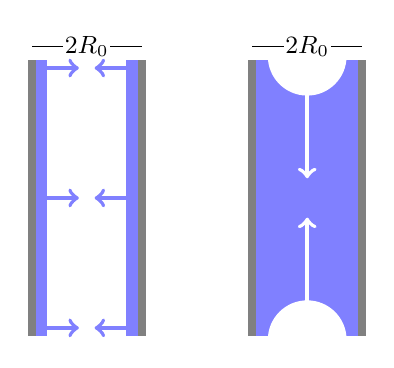
\begin{tikzpicture}[every node/.style = {font = \small},
                            pore/.style = {line width = 0.1cm, color = gray},
                            film/.style = {line width = 0.1cm, color = blue!50},
                            thick_film/.style = {line width = 0.3cm, color = blue!50},
                            graph_label/.style={color = gray, line width = 0.05cm},
                            pore_collapse/.style = {color = blue!50, line width = 0.07cm, ->},
                            MyArrow/.style={single arrow, draw, minimum width=8mm, minimum height=3mm,
                            inner sep=0mm, single arrow head extend=1mm},
                            fontscale/.style = {font=\relsize{#1}},
                            arrowstyle/.style = {scale=2},
                            MyArrow/.style={single arrow, draw, minimum width=8mm, minimum height=5mm, inner sep=0mm, single arrow head extend=1mm},
                            directed/.style={postaction={decorate,decoration={markings, mark=at position .65 with {\arrow[arrowstyle]{stealth}}}}}]
                \pgfdeclarelayer{bg}    % declare background layer
                \pgfdeclarelayer{bbg}    % declare backbackground layer
                \pgfsetlayers{bbg,bg,main}  % set the order of the layers (main is the standard layer)
                \begin{scope}
                \draw (0.4,3.67) -- (0,3.67);
                \draw (1,3.67) -- (1.4,3.67);
                \node at (0.7,3.67) {$2R_0$};
                \draw (3.2,3.67) -- (2.8,3.67);
                \draw (3.8,3.67) -- (4.2,3.67);
                \node at (3.5,3.67) {$2R_0$};
                    \foreach \Xcoor in {0,2.8}{
                    \draw[pore] (\Xcoor,3.5) -- (\Xcoor,0);
                    \draw[pore] (\Xcoor + 1.4,0) -- (\Xcoor + 1.4,3.5);}
                    \begin{pgfonlayer}{bg}
                        \draw[color = blue!50, ->, line width = 0.5mm] (.7,0.2) -- (.7,3.3);
                        %full pore with menisci
                        \fill[blue!50] (0.01,0) -- (0.01,3.5)  -- (1.39,3.5) -- (1.39,0) -- cycle ;
                        \fill[white] (1.2,3.55) -- (0.2,3.55) -- (0.2,-0.05) -- (1.2,-0.05) -- cycle;
                        \fill[blue!50] (2.81,0) -- (2.81,3.5)  -- (4.19,3.5) -- (4.19,0) -- cycle ;
                        \fill[white] (3,3.55) arc[start angle = -180, end angle = 0, radius=0.5] -- cycle;
                        \fill[white] (3,-0.05) arc[start angle = 180, end angle = 0, radius=0.5] -- cycle;
                        \draw[color=white,->, line width = 0.5mm] (3.5,3.5)--(3.5,2);
                        \draw[color=white,->, line width = 0.5mm] (3.5,0)--(3.5,1.5);
                        \foreach \Y in {.1,3.4,1.75}{
                        \draw[color=blue!50,->, line width = 0.5mm] (.1,\Y)--(.6,\Y);
                        \draw[color=blue!50,->, line width = 0.5mm] (1.3,\Y)--(.8,\Y);}
                        %full pore
                    \end{pgfonlayer}
                \end{scope}
              \end{tikzpicture}
              \label{fig:open-pore-process}
            }
    \caption{Menisci of the condensation and evaporation processes within a closed pore \protect\subref{fig:closed-pore-process} and an open pore \protect\subref{fig:open-pore-process}. For a closed pore, condensation and evaporation both occur at quilibrium pressure yielding spherical menisci. In contrast, the condensation in an open pore occurs at spinodal pressure with a cylindrical meniscus. The evaporation remains behaves unchanged occuring at equilibrium pressure.}
    \label{fig:pore-cond-evap-model}
\end{figure}
\end{document}
